We begin by considering the phenomenon of increasing efficiency in repeated reference games: speakers use detailed descriptions at the outset but converge to an increasingly compressed shorthand while remaining understandable to their partner.
While this phenomenon has been extensively documented, to the point of serving as a proxy for measuring common ground, it has continued to pose a challenge for models of communication.
For example, one possibility is that speakers coordinate on meaning through priming mechanisms at lower levels of representation, as proposed by influential  \emph{interactive alignment} accounts \cite{pickering2004toward, pickering2006alignment, garrod2009joint}.

  \begin{figure*}
\centering
    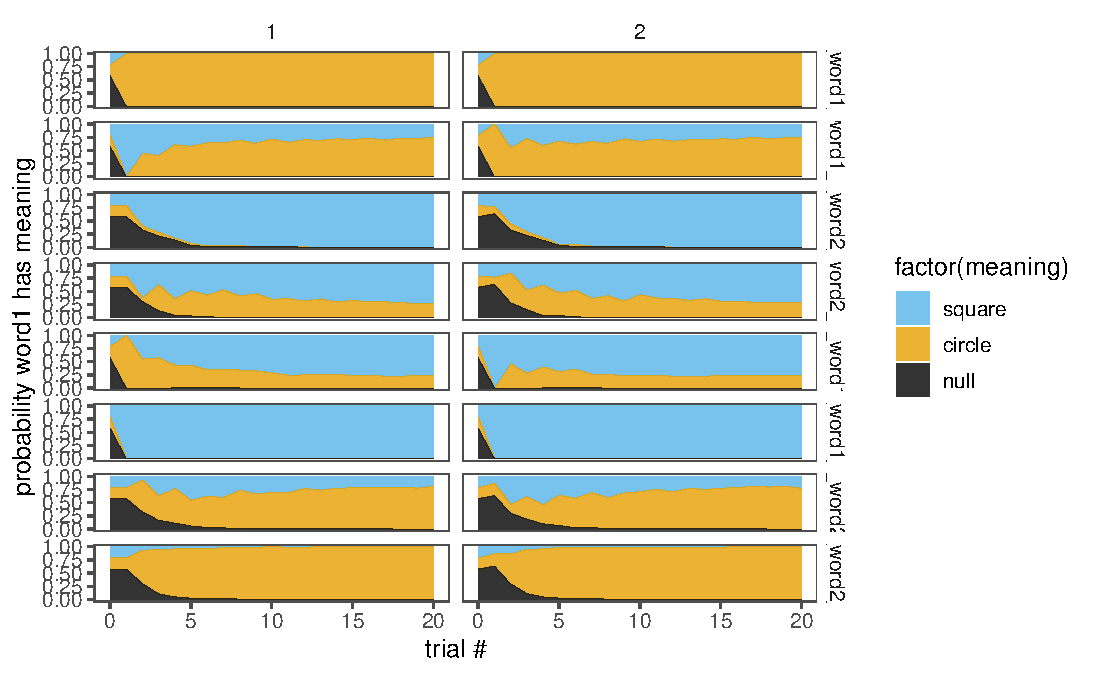
\includegraphics[scale=.9]{sec1-arbitrariness}
    \vspace{1em}
  \caption{\emph{Path-dependence of conventions.} The trajectory of each agent's beliefs about $\phi(u_1)$ in Simulation 1.1 are shown following all possible outcomes of the first trial. The top four rows are cases where the listener happened to correctly choose the target. In these cases, agents condition on the same data and rapidly converge on a system of meaning consistent with this feedback, e.g. when $u_1$ was successfully used to refer to the circle (shown in orange), both agents subsequently believe that $u_1$ means \emph{circle}. The bottom four rows show cases where the listener initially chooses the incorrect object. In these cases, the agents condition on different data (reflected in diverging beliefs on the second trial) but later recover from this mis-coordination.}
  \label{fig:path-dependence}
\end{figure*}

\begin{figure*}[b]
\centering
    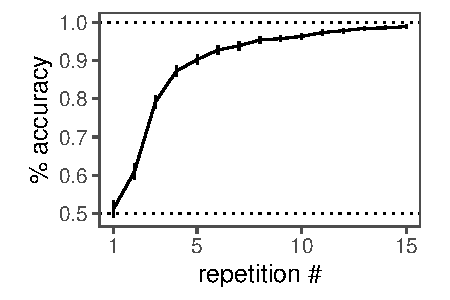
\includegraphics[scale=1.1]{sec1-convergence.pdf}
        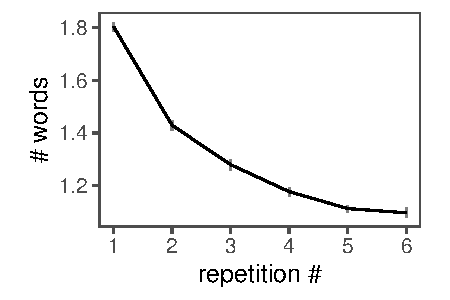
\includegraphics[scale=1.1]{sec1-efficiency}
  \caption{\emph{Pairs of agents learn to successfully coordinate on efficient ad hoc conventions over repeated interactions.} Results from 1000 simulated trajectories in (A) Simulation 1.1 and (B) Simulation 1.2 \ks{Think you need to explain the differenc ebetween these two simulations (briefly!) in the caption}. Error bars are bootstrapped 95\% CIs within each block of two trials.}
  \label{fig:sec1model}
\end{figure*}




While low-level priming may be at play in repeated reference tasks, especially when listeners engage in extensive dialogue or alternate roles, it is not clear why priming would cause descriptions to get shorter as opposed to aligning on the same initial description.
Furthermore, priming alone cannot explain why speakers still converge to more efficient labels even when the listener is prevented from saying anything at all and only minimal feedback is provided showing that the listener is responding correctly \cite{KraussWeinheimer66_Tangrams}; conversely, speakers continue using longer descriptions when they receive non-verbal feedback that the listener is repeatedly making errors \cite<see also>{hawkins2020characterizing}.
In these cases, there are no linguistic features available for priming or alignment mechanisms.
Explaining when and why speakers believe that shorter descriptions will suffice requires a mechanism for coordination on meaning even given sparse, non-verbal feedback.

Another possibility is that speakers coordinate on meaning using some some lexical update rule that makes utterances more likely to be produced after communicative successes and less likely after communicative failures, such as a variant on the Roth-Erev reinforcement learning rule \cite{erev1998predicting} adopted by a variety of agent-based models \cite{steels_self-organizing_1995,barr_establishing_2004,young_evolution_2015}.
While reinforcement is a powerful mechanism for allowing groups to reach consensus, it is not clear why a newly initialized speaker would prefer to produce longer utterances over shorter utterances, or, if this bias was built-in, how simply reinforcing initially long descriptions could lead utterances to get shorter. 
In the rare cases that some form of reduction has been investigated in this family of models (e.g. as in the phenomenon of phonological erosion), the process has been hard-coded as an $\epsilon$ probability of speakers dropping a random token at each point in time \cite{beuls2013agent,steels2016agent}.

Such random dropping, however, is an unsatisfying explanations for several reasons.
First, it formalizes a reductive explanation of efficiency in terms of speaker-internal noise (or laziness) that dates back to the early literature on repeated reference games.
Control experiments by \citeA{HupetChantraine92_CollaborationOrRepitition} were designed to test this possibility \cite<see also>{GarrodFayLeeOberlanderMacLeod07_GraphicalSymbolSystems}. 
Participants were asked to repeatedly refer to the same targets for a \emph{hypothetical} partner to see later, such that any effects of familiarity or repetition on the part of the speaker were held constant with the interactive task. 
No evidence of reduction was found, and in some cases utterances actually grew longer.
This accords with observations in multi-partner settings by \citeA{wilkes-gibbs_coordinating_1992}, which we explore further in \textbf{P2}: it is difficult to explain why a speaker who only shortened their descriptions due to an $\epsilon$-noise process would suddenly switch back to a longer utterance when their partner is exchanged.
Whatever drives efficiency cannot be explained through speaker laziness, it must be a result of the \emph{interaction} between partners.

In this section, we argue that our Bayesian account provides a rational explanation for increasing efficiency in terms of the inferences made by speakers across repeated interaction.
Given that this phenomenon arises in purely dyadic settings, it also provides an opportunity to explore more basic properties of the first two capacities formalized in our model (representing \emph{uncertainty} and \emph{partner-specific learning}) before introducing hierarchical generalization in the next section. 
In brief, we show that increasing efficiency is a natural consequence of the speaker's tradeoff between informativity and parsimony (Eq.~\ref{eq:marginalized}), given their inferences about the listener's language model. 
For novel, ambiguous objects like tangrams, where speakers do not expect strong referential conventions to be shared, longer initial descriptions are motivated by high initial uncertainty in the speaker's lexical prior $P(\phi_k | \Theta)$. 
Proposing multiple descriptors is a hedge against the possibility that any particular meaning is not shared by the listener.
As the interaction goes on, the speaker obtains feedback $D_k$ from the listener responses and updates their posterior beliefs $P(\phi_k | D_k)$ accordingly. 
As uncertainty gradually decreases, they are able to achieve the same expected informativity with shorter, more efficient messages. 

\subsection{Simulation 1.1: Pure coordination}


We build up to our explanation of increasing efficiency by first exploring a simpler simulation.
This first simulation demonstrates the most fundamental desideratum for any model of \emph{ad hoc} coordination: agents are able to coordinate on a communication system in the absence of shared priors. 
For clarity, we consider the simplest possible reference game with two objects, $\mathcal{O} = \{o_1, o_2\}$, where the speaker must choose between two one-word utterances $\mathcal{U} = \{u_1, u_2\}$ with equal production cost. 
We initialize agents with uniform priors, $\phi(u_i) \sim \textrm{unif}\{o_1, o_2\}$, for all $u_i \in \mathcal{U}$.

The first step proceeds as follows, illustrated in Fig. \ref{fig:path-dependence}.
Suppose the target object on the first round is $o_1$.
Due to uniform priors, both utterances are equally likely to apply to either object, and because each utterance is equally (un)informative, the speaker effectively samples an utterance at random $u~\sim~S(u|o_1)$.
Suppose it is $u_1$.
They may then observe the listener's selection of an object $o \sim L(o | u_1)$ --- say, $o_1$, a correct response.
Finally, they may use the observed pair $D = \{u_1, o_1\}$ to update their beliefs about the listener's true lexicon $P(\phi | D)\propto L_1(o_1 | u_1, \phi)P(\phi)$.
The listener is similarly able to update their beliefs about the speaker's true lexicon $P(\phi | D)\propto S_1(u_1 | o_1, \phi)P(\phi)$. 
Both agents then proceed to the next trial, where they use this updated posterior distribution to produce or interpret language.
\begin{figure*}
\centering
    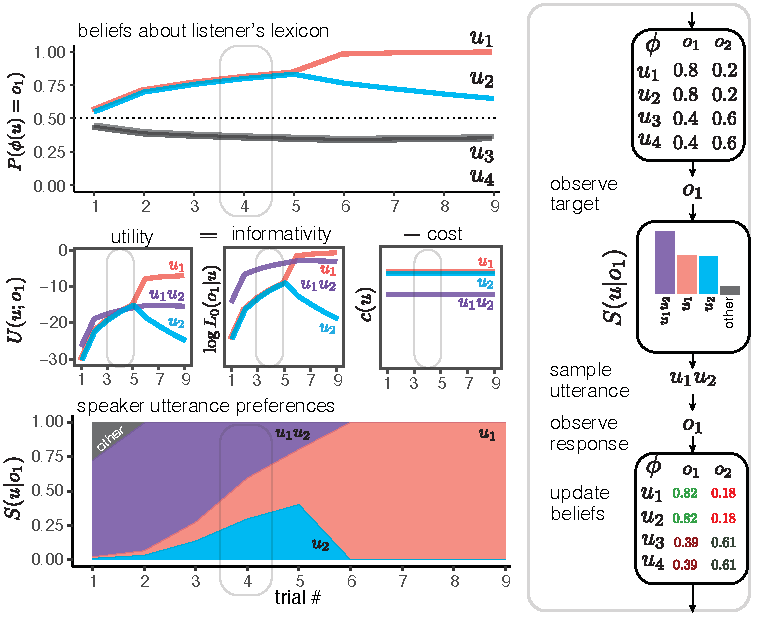
\includegraphics[scale=1.5]{sec1-reduction_example}
    \vspace{1em}
  \caption{\emph{Schematic of speaker for first trial of Simulation 1.2.} The speaker begins with uncertainty about the meanings in the listener's lexicon (e.g. assigning 55\% probability to the possibility that utterance $u_1$ means object $o_1$.) A target $o_1$ is presented, and the speaker samples an utterance from the distribution $S(u|o_1)$. Finally, they observe the listener's response and update their beliefs. Due to the compositional semantics of the utterance $u_1u_2$, the speaker becomes increasingly confident that both component primitives, $u_1$ and $u_2$, apply to object $o_1$ in their partner's lexicon.}
  \label{fig:sec1efficiency}
\end{figure*}

To examine how the dynamics of this process unfold over multiple rounds, we simulated 1000 trajectories, each of which was 30 trials in length, organized into 15 blocks.
Agents swapped speaker and listener roles on each trial, and we randomized the target sequence within each block \ks{I found this wording a bit confusing; there are two meanings, so basically this is each block they see them both in random order?}.
This simulation was conducted at soft-max optimality parameter values $w_L = w_S = 16$ and memory discounting parameter $\beta = 0.8$, but see Appendix Fig.~\ref{fig:arbitrariness_grid} for an exploration of behavior at other values.
Agents were initialized with the same priors in every trajectory, such that trajectories only diverged when different actions happen to be sampled.
For example, if the speaker samples $u_2$ instead of $u_1$ on the first trial, or if the listener makes an error by choosing $o_2$, then they will subsequently condition on these observations instead, leading to different downstream beliefs and behavior (see Fig. \ref{fig:path-dependence} for the average trajectories resulting from all possible combinations of speaker and listener choices on the first trial).

We highlight several key results from these simulations.
First, most fundamentally, the communicative success of the dyad rises over the course of interaction; the listener is able to more accurately select the true target object (see Fig.~\ref{fig:sec1model}A). 
Second, the initial symmetry between the meanings is broken by initial choices, leading to \emph{arbitrary} but \emph{stable} mappings in future rounds.
This can be seen by examining the path-dependence of beliefs, following all possible outcomes of the initial trial (see Fig.~\ref{fig:path-dependence}). 
Third, we see the clear influence of mutual exclusivity via Gricean pragmatic reasoning (see \emph{Bias against ambiguity} above): agents also make inferences about \emph{unheard} utterances. 
Observing $D = \{(u_2, o_1)\}$ also provides evidence that $u_1$ is \emph{not} a good fit for $o_1$ (e.g.~see the third row of Fig.~\ref{fig:path-dependence}).
%Fourth, conventions may form based on \emph{failed references} as well as successful ones: if the speaker intends $o_1$ and says $u_1$, but then the listener incorrectly picks $o_2$, the speaker will take this as evidence that $u_1$ actually means $o_2$ in their partner's lexicon and become increasingly likely to use it that way on subsequent rounds.

\subsection{Simulation 1.2: Efficiency}

Next, we show how our inferential model explains speakers' gains in efficiency over multiple interactions. 
For efficiency to change at all, speakers must be able to produce utterances that vary in length. 
For this simulation, we therefore extend the grammar\ks{model?} to allow for multi-word utterances by allowing speakers to combine together multiple primitive utterances with disjunctive semantics.
Specifically, we consider a scenario with the same two objects as in Simulation 1.1, but giving the speaker four primitive utterances $\{u_1, u_2, u_3, u_4\}$ instead of only two. 
Critically, the meaning of longer utterances are derived compositionally from these primitives using the maximum $t$-conorm\footnote{We focus on disjunction as one of the simplest operations to construct longer, non-atomic utterances from primitives. See also \citeA{SteinertThrelkeld16_CompositionalSignaling} who consider the operation of negation.}:
$$\mathcal{L}_\phi(u_iu_j, o) = \max\{\mathcal{L}_\phi(u_i, o) , \mathcal{L}_\phi(u_j, o)\}$$
\ks{This bit of maths confused the bejesus out of me until I eventually realised (I think?) that $\mathcal{L}_\phi(u_i, o)$ is binary, i.e. it's either 1 or 0 for any particular lexicon. I was looking at these plus the probabilities in fig 5 and wondering what on earth stringing a couple of signals together was going to add. A brief e.g. might help.}

While we established in the previous section that successful \emph{ad hoc} conventions can emerge even in a state of pure uncertainty, human participants in repeated reference games typically bring some prior expectations about language into the interaction.
For example, a participant who hears `ice skater' on the first round of a task with tangram stimuli may be more likely to select some objects more than others while still having substantial uncertainty about the intended target.
This observation is key to understanding why speakers may initially use longer utterances in repeated reference games with ambiguous stimuli. 
Under a completely uniform prior, where all words are expected to be equally meaningless to one's partner, longer utterances have no additional value. 
Under a completely concentrated prior, where there already exists a strong convention for a short label, that label would suffice and a longer utterances is redundant.
We thus initialize both agents with weak lexical beliefs
$$P(\phi(u_1) = o_1) = P(\phi(u_2) = o_1) = 0.55$$ 
$$P(\phi(u_3) = o_1) = P(\phi(u_4) = o_1) = 0.45$$
and show how our model predicts an initial preferences for long utterances but increasing preferences for shorter utterances given communicative success.

%\begin{figure}[b]
%\centering
%  \caption{\emph{Agent converge on more efficient utterances over repeated interactions.} Error bars are bootstrapped 95\% CIs across 1000 simulated trajectories.}
%  \label{fig:sec1efficiency}
%\end{figure}


\begin{figure*}[t]
\centering
    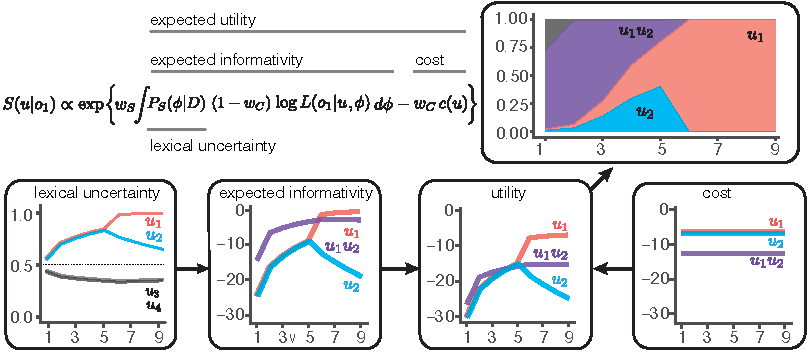
\includegraphics[scale=1.2]{sec1-reduction_schematic}
    \vspace{1em}
  \caption{\emph{Internal state of speaker in example trajectory from Simulation 1.2.} Each term of the speaker's utility (Eq. \ref{eq:marginalized}) is shown throughout an interaction. When the speaker is initially uncertain about meanings (far left), the longer utterance $u_1u_2$ has higher expected informativity (center-left) and therefore higher utility (center-right) than the shorter utterances $u_1$ and $u_2$, despite its higher cost (far-right). As the speaker observes several successful interactions, it updates its beliefs and becomes more confident about the meanings of the component lexical items $u_1$ and $u_2$. As a result, more efficient single-word utterances gradually gain in utility as cost begins to dominate the utility. On trial 5, $u_1$ is sampled, breaking the symmetry between utterances.}
  \label{fig:sec1internals}
\end{figure*}

As in Simulation 1.1, we simulated 1000 trajectories of dyadic interaction between agents.
Target objects were randomly sampled on each trial, agents swapped roles, and the agents' lexical posteriors $P(\phi | D)$ were computed after each trial using exact enumeration. 
Utterance cost is defined to be the number of `words' in an utterance, so $c(u_1) =1$ and $c(u_1u_2)=2$.
Results are shown in Fig.~\ref{fig:sec1model}B.
As in repeated reference games between human participants (e.g. Fig.~\ref{fig:clark92}), our speaker agent initially prefers longer utterance (mean length $\approx 1.5$ on first block) but rapidly converges to shorter utterances after several repetitions (mean length $\approx 1$ on final block).

To illustrate in detail how our model derives this phenomenon as a consequence of rational inference, we walk step-by-step through a single trial (Fig. \ref{fig:sec1efficiency}).
Consider a speaker who wants to refer to object $o_1$. 
They expect their partner to be slightly more likely to interpret their language using a lexicon in which $u_{1}$ and $u_{2}$ apply to this object, due to their weak initial biases. 
However, there is still a reasonable chance ($p=0.45$) that either $u_1$ or $u_2$ alone will be interpreted to mean $o_2$ by their partner, which would lead to an incorrect response. 
Thus, it is more informative to produce the longer utterance $u_{1}u_{2}$ to hedge against this possibility, despite its higher production cost. 

To see why this is the case, consider the expected informativity of the utterance under different possible listener lexicons.
The possibility with highest probability is that both $u_1$ and $u_2$ will mean $o_1$ in the listener's lexicon ($p = 0.55^2 \approx 0.3$), in which case the listener will correctly identify the target with high probability.
The possibility that both $u_1$ and $u_2$ will mean $o_2$ in the listener's lexicon is only $p=0.45^2 \approx 0.2$, leading the listener to erroneously select $o_2$ with high probability. 
In the mixed cases, where just one of $u_1$ or $u_2$ means $o_2$ in the listener's lexicon ($p = 2 \cdot 0.45 * 0.55 \approx 0.5$), the listener will choose between the objects at chance, which yields an intermediate informativity.
When expected informativity is calculated across these outcomes, it is more valuable to produce the longer disjunction than the shorter component utterances.
Finally, upon observing the listener's response to the disjunction (say, $o_1$), the speaker becomes more confident that the component utterances $u_1$ and $u_2$ mean $o_1$ in their updated posterior over the listener's lexicon.
This credit assignment to individual lexical items is a consequence of the compositional meaning of longer utterances in our simple grammar.

Fig.~\ref{fig:sec1internals} shows the trajectories of internal components of the speaker utility as the interaction continues.
We assume for illustrative purposes that $o_1$ continues to be the target on each trial and the same agent continues to be the speaker.
As the posterior probability that individual primitive utterances $u_1$ and $u_2$ independently mean $o_1$ increases (far left), the marginal gap in informativity between the disjunction and the shorter components gradually decreases (center left).
As a consequence, production cost increasingly dominates the utility (center-right). 
After several trials of observing a successful listener response given the disjunction, the utility of the shorter utterances reaches parity with the disjunction.
Once the speaker samples a shorter utterance (e.g. $u_1$), the symmetry collapses and that utterance remains most probable in future rounds, allowing for a stable and efficient \emph{ad hoc} convention. \ks{Doesn't this suffer from the same criticism you level at Beule and Steels, namely any word could be dropped?}
Thus, increasing efficiency is derived as a rational consequence of inference about the listener's lexical.
For these simulations, we used $w_S = w_L = 7, w_c = 11, \beta=0.8$ but the qualitative reduction effect is found over a range of different parameters (see Appendix Fig. \ref{fig:conjunction_grid}). 
%\paragraph{Model comparison}
%
%Here we compare this model to several simpler baselines to establish which components of the model are necessary and sufficient for the desired behavior.
%
%\rdh{e.g., no pragmatics, pragmatics only in learning rule or only in decision rule instead of both, simpler pragmatics (reasoning about $L_0$ instead of $L_1$), point estimate instead of uncertainty, effect of different parameter regimes.} 
%
%\rdh{It may also be useful to explicitly show that the simpler Roth-Erev RL updating from this literature doesn't reduce, or even better show that this kind of simpler update rule is equivalent to something within our framework as a point estimate representation with maximum likelihood or something...?}

%In the limit, it doesn't matter whether you have pragmatics in both learning rule or decision rule. 
%In case where it's only in production rule, you'll produce the data with the necessary biases in learning.



\subsection{Discussion}

The simulations presented in this section aimed to establish a rational explanation for feedback-sensitive increases in efficiency over the course of \emph{ad hoc} convention formation.
Speakers initially hedge their descriptions under uncertainty about the lexical meanings their partner is using, but are able to get away with less costly components of those descriptions as their uncertainty decreases.
Our explanation recalls classic observations about \emph{hedges}, expressions like \emph{sort of} or \emph{like}, and morphemes like \emph{-ish}, that explicitly mark provisionality, such as \emph{a car, sort of silvery purple colored} \cite{Fraser10_Hedging,MedlockBriscoe07_HedgeClassification}.
\citeA{BrennanClark96_ConceptualPactsConversation} counted hedges across repetitions of a repeated reference game, finding a greater occurrence of hedges on early trials than later trials and a greater occurrence under more ambiguous contexts.
While our model does not explicitly produce hedges, it is possible to understand this behavior as an explicit or implicit marker of the lexical uncertainty theorized by our account.

We have already discussed why this phenomenon poses a challenge for the simple model-free reinforcement learning models in the literature --- namely, that successful listener feedback only reinforces long utterances with no mechanism for shortening them.
This observation is not intended to rule out the entire family of reinforcement learning approaches: it is plausible that more sophisticated \emph{model-based} reinforcement learning algorithms are flexible enough to account for the phenomenon.
For instance, hierarchical architectures that appropriately incorporate compositionality or incrementality into the speaker's production model may be able to reinforce component parts of longer utterances in the shared history \cite<e.g>{hawkins2019continual}.
However, such an approach would bring these models much closer to the features of our proposal than to the model-free agents in the existing literature.
We return to this question in our discussion of the scalability of our model in the General Discussion.

Finally, our explanation of reduction in this section is consistent with recent analyses of exactly \emph{what} gets reduced, using a large corpus of repeated reference games \cite{hawkins2020characterizing}.
These analyses found that entire modifying clauses are more likely to be dropped at once than expected by random corruption, and function words like determiners are mostly dropped as parts of larger noun phases or prepositional phrases rather than omitted on their own.
In other words, speakers apparently begin by combining multiple descriptive labels and collapse to one of these labels, rather than randomly dropping words because the listener can be expected to recover the intended longer utterance, as predicted by a ``noisy channel'' model.
This claim is further supported by early hand-tagged analyses by \citeA{Carroll80_NamingHedges}, which found that in three-quarters of transcripts from \citeA{krauss_changes_1964} the conventions that participants eventually converged upon were prominent in some syntactic construction at the beginning, often as a head noun that was initially modified or qualified by other information. 
While our simulation only considered two-word descriptions with homogenous uncertainty over the components, it is likely that the semantic components of real initial descriptions have more heterogeneous uncertainty: the head noun may be chosen due to a higher prior probability of being understood by the listener than other components of the initial description, thus predicting asymmetries in reduction. \ks{So this is dealing with the Beule and Steels thing now, but it reads as relatively weak here}

